% Source: Lecture12.pdf, pages 1-7. Title on the source: "Lecture 12: Ising model in 2D".
\lecture{12}

In the previous lecture, we discussed the Kramers--Wannier derivation of $T_c$ in the Ising model on
the square lattice. Recall that since the square lattice is bipartite, we could, with no loss of
generality, assume $J>0$, hence $K = \beta J>0$. We used a low-temperature expansion in the variable
$z = e^{-2K}$ and a high-temperature expansion in the variable $v = \tanh K$, and showed a 1--1
correspondence between the terms in these expansions. The expansions extend from $T = \infty$ (i.e.\
$v = 0$) down and from $T = 0$ (i.e.\ $z = 0$) up, and meet at a unique point, which is the critical
point $T_c$. Equating the series for the partition function at $T = T_c$ (since the phase transition is
continuous), we set $z = v$. Now $v = (1-z)/(1+z)$, so this yields the equation
$z = (1-z)/(1+z)$, i.e.\ $z^2+2z-1 = 0$, with solutions $z = -1\pm\sqrt2$, of which only
$-1+\sqrt2$ is physical, since $-1-\sqrt2<0$, but $z = e^{-2K}$ is non-negative. So the critical point
is at $z = z_c = -1+\sqrt2$. Solving for $K_c$: $z_c = e^{-2K_c}$, $e^{-2K_c} = \sqrt2-1$,
$-2K_c = \ln(\sqrt2-1)$, so
\begin{equation}
  K_c = -\frac{1}{2}\ln(\sqrt2-1) = +\frac{1}{2}\ln\left(\frac{1}{\sqrt2-1}\right) = \frac{1}{2}\ln(\sqrt2+1) = 0.4407 .
\end{equation}
Note that we can equivalently obtain this result by using
$\operatorname{arctanh}x = (1/2)\ln[(1+x)/(1-x)]$:
with $v = v_c = \tanh K_c = \sqrt2-1$,
\begin{align}
  K_c &= \operatorname{arctanh}v_c = \frac{1}{2}\ln\left(\frac{1+v_c}{1-v_c}\right)
       = \frac{1}{2}\ln\left(\frac{1+(\sqrt2-1)}{1-(\sqrt2-1)}\right)\nonumber\\
      &= \frac{1}{2}\ln\left(\frac{\sqrt2}{2-\sqrt2}\right) = \frac{1}{2}\ln\left(\frac{1}{\sqrt2-1}\right) = \frac{1}{2}\ln(\sqrt2+1).
\end{align}
Then, with $K = J/(\kB T)$, solving for $T_c$,
\begin{equation}
  \kB T_c = \frac{J}{K_c} = \frac{J}{\frac{1}{2}\ln(\sqrt2+1)} = 2.269\,J .
\end{equation}
As we discussed earlier, this is lower than the MFT estimate, $K_{c,\text{MFT}} = 1/\Delta = 1/4$
here, i.e.\ $\kB T_{\text{MFT}} = J/K_{c,\text{MFT}} = 4J$. We saw the Peierls Theorem with plausible
estimates for the path branching parameter $c$ yields a value of $T_c$ comparable to the exact value:
$\kB T_c\simeq 2J/\ln c$; $2\le c\le 3$, and with $c = 2.5$, $\kB T_c = 2J/\ln(2.5) = 2.2J$.

\subsection{The 2D Ising model and its exact solution}
\subsubsection*{The Ising model in two dimensions}

We now proceed to discuss some relevant results for the Ising model on 2D lattices. We focus on the
square lattice for definiteness; the critical behavior is the same for the model with ferromagnetic
coupling $J>0$ on all 2D lattices. This is easy to understand: as $T\nearrow T_c$ or $T\searrow T_c$,
the correlation length $\xi\to\infty$, and hence short-distance details of lattice structure become
irrelevant; e.g.\ it does not matter for the critical behavior whether the lattice is sq, tri, hc, or
some other regular lattice. This property will also be evident in the context of the renormalization
group, RG. On a bipartite lattice such as the sq and hc lattices, because of the isomorphism relating
the FM ($J>0$) and AFM ($J<0$) signs of $J$, with the corresponding mapping of uniform
$\leftrightarrow$ staggered magnetization, it follows that the critical behavior of the model with
$J<0$ is also independent of the lattice type.

However, it is not, in general, true that the FM and AFM versions of the model have the same critical
behavior on a non-bipartite lattice, since the AFM case may entail frustration. An example is the
Ising AFM on the triangular lattice, where the frustration removes the finite-temperature phase
transition.

\paragraph{Some helpful relations.}

Besides $v = (1-z)/(1+z)$, $z = (1-v)/(1+v)$, also:
\begin{align}
  \sinh K &= \frac{v}{\sqrt{1-v^2}} = \frac{1-z}{2\sqrt z}, &
  \sinh(2K) &= 2\sinh K\cosh K = \frac{2v}{1-v^2} = \frac{1-z^2}{2z},\\
  \cosh K &= \frac{1}{\sqrt{1-v^2}} = \frac{1+z}{2\sqrt z}, &
  \cosh(2K) &= \cosh^2K+\sinh^2K = \frac{1+v^2}{1-v^2} = \frac{1+z^2}{2z}.
\end{align}
N.B.: $\sinh 2K\to 1$ as $K\to K_c$, which can be seen with either expression as a function of $z$ or
$v$; e.g., with $z_c = \sqrt2-1$,
\begin{equation}
  \sinh 2K_c = \frac{(1+z_c)(1-z_c)}{2z_c} = \frac{\sqrt2(2-\sqrt2)}{2(\sqrt2-1)} = 1 .
\end{equation}
The quantity $\tilde k_>\equiv\sinh^22K$ will appear in correlation functions at $T>T_c$ and
$\tilde k_<\equiv1/\tilde k_> = 1/(\sinh^22K)$ in correlation functions at $T<T_c$. These
are equal and equal to 1 at $T_c$: $\tilde k_< = \tilde k_> = 1$ at $T_c$.

The quantity
\begin{equation}
  \kappa\equiv\frac{2\sinh 2K}{\cosh^22K}
\end{equation}
occurs in the specific heat. With the identity $\cosh^2x-\sinh^2x = 1$, one has
$\cosh^22K_c = 1+\sinh^22K_c = 2$, so $\kappa_c = 2\cdot 1/2 = 1$. As $K\to 0$ and
$K\to\pm\infty$, $\kappa\to 0$, so $\kappa$ reaches its maximal value of 1 at $K_c$.

\begin{diagram}
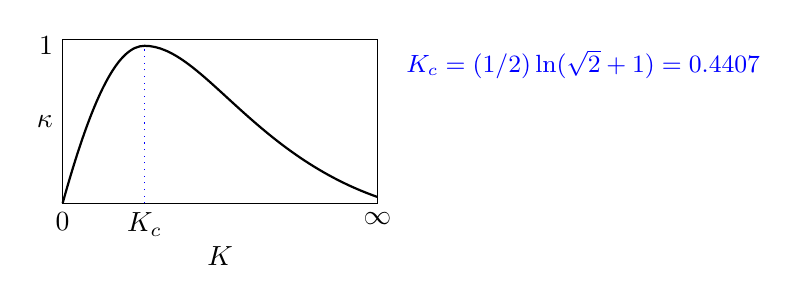
\begin{tikzpicture}[scale=0.8]
  \draw (0,0) rectangle (5,2.6);
  \draw[thick] (0,0) .. controls (0.5,1.8) and (0.9,2.5) .. (1.3,2.5) .. controls (2.2,2.5) and (3,0.8) .. (5,0.1);
  \draw[dotted,blue] (1.3,0) -- (1.3,2.5);
  \node[left] at (0,1.3) {$\kappa$};
  \node[below] at (0,0) {$0$}; \node[below] at (1.3,0) {$K_c$}; \node[below] at (5,0) {$\infty$};
  \node[below=12pt] at (2.5,0) {$K$};
  \node[left] at (0,2.5) {$1$};
  \node[blue,anchor=west,font=\small] at (5.3,2.2) {$K_c = (1/2)\ln(\sqrt2+1) = 0.4407$};
\end{tikzpicture}
\diagramcaption{The elliptic modulus $\kappa$ as a function of $K$.}
\end{diagram}

\subsubsection*{Exact results and their history}

The 2D Ising model was important in the historical development of stat.\ mech.\ and the theory of
critical phenomena because one could, at least for zero external magnetic field, $H = 0$, calculate
exact closed-form expressions for some (not all) thermodynamic quantities, in particular the Gibbs
free energy $G(T,H=0)$. This was calculated in 1944 by L.~Onsager. From this one can calculate the
internal energy $U(T,H=0)$ and the specific heat capacity $C_H(T,H=0)$ [L.~Onsager, Phys.\ Rev.\
\textbf{65}, 117 (1944)]. One finds that $C$ has a logarithmic divergence at $T_c$ (so
$\alpha = \alpha' = 0$). The spontaneous magnetization $M_{sp}$ was calculated by C.N.~Yang in 1952
[C.N.~Yang, Phys.\ Rev.\ \textbf{85}, 808 (1952)], yielding the critical exponent $\beta = 1/8$.
These values of critical exponents were of great interest because they differed from the predictions
of LG and MFT, which were that $C$ has a discontinuity at $T_c$ and that the critical exponent for the
magnetization is $\beta_{\text{MFT}} = 1/2$.

These calculations were initially for the square lattice and were later extended to other 2D lattices,
which gave the same values for the exponents, thereby providing analytical support for universality of
critical behavior, independent of lattice structure (in the absence of frustration). This was also very
important, since experiments on magnetic phenomena in different Ising-like (uniaxial) materials had
observed this universality (as had experiments on critical phenomena in liquid--gas systems; recall the
plot from Guggenheim showing the same $\beta\sim 0.35$ for the critical point in various gases). No
closed-form solutions have ever been obtained for the initial magnetic susceptibility
$\chi = \left.\partial M/\partial H\right|_{H=0}$ or for any of these quantities in a nonzero physical
external magnetic field $H$. However, later, a procedure was worked out for calculating
$\ev{\sigma_{\mathbf 0}\sigma_{\mathbf r}} = \ev{\sigma_{(0,0)}\sigma_{(i,j)}}$ by Montroll, Potts, and
Ward, and this was used to study the asymptotic behavior of the spin--spin correlation function to
infer the critical exponents $\nu$ and $\nu'$ describing the divergence in $\xi$ as $T\to T_c$ (recall
$\ev{\sigma_{\mathbf 0}\sigma_{\mathbf r}}_{\text{conn.}}\sim e^{-r/\xi}$ as $|\mathbf r| = r\to\infty$).
It was found that $\nu = \nu' = 1$. A similar study of the spin--spin correlation function at $T_c$
yielded $\eta = 1/4$ (recall $\ev{\sigma_{\mathbf 0}\sigma_{\mathbf r}}\sim 1/r^{d-2+\eta}$ at
$T = T_c$).

Although most experimental measurements of critical phenomena, such as liquid--gas systems (which are in
the Ising universality class) and magnetic systems, are 3D rather than 2D, these exact results for the
critical exponents of the 2D Ising model were valuable as a demonstration of non-MFT,
non-Landau--Ginzburg critical behavior.

\subsection{Free energy, internal energy and specific heat}
\subsubsection*{The free energy}

The reduced dimensionless free energy $f = f(T,H=0)$, where $G(T,H) = -\kB Tf(T,H)$, can be calculated
by a transfer matrix method similar to, but more complicated than, our use of this method in the 1D
model. The result for $f$ (for the square lattice) is
\begin{equation}
  f = \ln 2 + \frac{1}{2}\int_{-\pi}^{\pi}\frac{\dd\theta_1}{2\pi}\int_{-\pi}^{\pi}\frac{\dd\theta_2}{2\pi}
      \ln\left[L(\theta_1,\theta_2)\right],
\end{equation}
where $L = L(\theta_1,\theta_2)$ is
\begin{equation}
  L = \cosh^2(2K) - \sinh(2K)\cdot\mathcal{P},\qquad\text{with}\quad \mathcal{P} = \cos\theta_1+\cos\theta_2 .
\end{equation}
Over the range of integration, $\mathcal P$ varies from $-2$ to $+2$. The free energy $f$ has a
non-analyticity where $L = 0$. Now $\cosh^22K_c = 2$ and
$\sinh 2K_c = \begin{cases}1 & \text{for FM}\\ -1 & \text{for AFM}\end{cases}$, so one sees that this
non-analyticity occurs at $K = \pm K_c$:
\begin{align*}
  \text{FM case } J>0:&\quad L = 2 - 1\cdot\mathcal P = 0\quad\text{if } \mathcal P = 2,\\
  \text{AFM case } J<0:&\quad L = 2 - (-1)\cdot\mathcal P = 0\quad\text{if } \mathcal P = -2.
\end{align*}
As $T\to\infty$, $K\to 0$, $L\to 1$, $\ln L\to 0$, so $f\to\ln 2$. This reflects the fact that when
$\beta = 0$, the spin--spin interaction has no effect, so $Z = 2^N$,
$f = \lim_{N\to\infty}(1/N)\ln Z = \ln 2$; spins are completely random. For the other limit, without
loss of generality, assume $J>0$, so $K>0$, the FM case. As $T\to 0$, the spins approach a completely
ordered state (all $+$ or all $-$), so in $Z = \sum_{\{\sigma_i\}}e^{K\sum_{e_{ij}}\sigma_i\sigma_j}$, the
argument of the exponential $\to K\cdot e(\Lambda) = K\cdot(\Delta/2)n(\Lambda) = K(\Delta_{sq}/2)N = 2KN$
(with $\Delta_{sq} = 4$), so
\begin{equation}
  Z\to 2e^{2KN},\qquad \ln Z = \ln 2 + 2KN,\qquad f = \lim_{N\to\infty}\frac{1}{N}\ln Z\to 2K .
\end{equation}
We see how the exact result agrees with this as $T\to 0$:
$\cosh^2(2K) = \left((e^{2K}+e^{-2K})/2\right)^2\to e^{4K}/4$, which dominates over
$\sinh 2K\to e^{2K}/2$, so the $\theta$-independent first term in $L$ dominates over the
$\theta$-dependent term and
\begin{equation}
  f\to\ln 2 + \frac{1}{2}\int_{-\pi}^{\pi}\frac{\dd^2\theta}{(2\pi)^2}\ln\left(\frac{e^{4K}}{4}\right)
  = \ln 2 + \frac{1}{2}(4K - 2\ln 2) = 2K,
\end{equation}
since $\int_{-\pi}^{\pi}\dd^2\theta/(2\pi)^2 = 1$.

It is also useful to express $f$ in terms of $z$ and $v$. Using $\cosh(2K) = (1+z^2)/(2z)$ and
$\sinh(2K) = (1-z^2)/(2z)$, with $\mathcal P = \cos\theta_1+\cos\theta_2$,
\begin{align}
  f &= \ln 2 + \frac{1}{2}\int_{-\pi}^{\pi}\frac{\dd^2\theta}{(2\pi)^2}\ln\left[\cosh^2(2K)-\sinh(2K)\mathcal P\right]\nonumber\\
    &= \ln 2 + \frac{1}{2}\int_{-\pi}^{\pi}\frac{\dd^2\theta}{(2\pi)^2}\ln\left[\frac{(1+z^2)^2}{(2z)^2}-\frac{(1-z^2)}{2z}\mathcal P\right]\nonumber\\
    &= \underbrace{\ln 2 - \ln(2z)}_{\ln 2-\ln 2-\ln(e^{-2K}) = 2K}
     + \frac{1}{2}\int_{-\pi}^{\pi}\frac{\dd^2\theta}{(2\pi)^2}\ln\left[(1+z^2)^2 - 2z(1-z^2)\mathcal P\right].
\end{align}
Although one cannot do both of the integrations, it is possible to do one. This gives $f$ in terms of a
single integral (HW):
\begin{equation}
  f = \ln\left(2\cosh(2K)\right) + \frac{1}{2}\int_0^\pi\frac{\dd\phi}{\pi}
      \ln\left[\frac{1+\sqrt{1-\kappa^2\sin^2\phi}}{2}\right],
\end{equation}
where, as above, $\kappa = 2\sinh(2K)/\cosh^2(2K)$ ($\kappa\to-\kappa$ as $J\to-J$, FM vs.\ AFM sign). This again exhibits a non-analyticity at
$\kappa = 1$, where the argument of the square root can vanish.

\subsubsection*{Internal energy and specific heat}

Then, $\bar U = -\partial f/\partial \beta = -J\partial f/\partial K$ $\Rightarrow$
\begin{equation}
  \bar U = -J\coth(2K)\left[1 + \frac{2}{\pi}\left(2\tanh^2(2K)-1\right)K(\kappa)\right],
\end{equation}
where
\begin{equation}
  K(\kappa) = \int_0^{\pi/2}\frac{\dd\omega}{\sqrt{1-\kappa^2\sin^2\omega}}
\end{equation}
is the complete elliptic integral of the first kind and $\kappa$ is the elliptic modulus. Here we follow
standard mathematical notation; do not confuse this $K(\kappa)$ with $K = \beta J$. Note that $K(\kappa)$
only depends on $\kappa^2$.

An important property of $K(\kappa)$ is that $K(\kappa)$ diverges logarithmically as $\kappa^2\to 1$.
Since $K(\kappa)$ only depends on $\kappa^2$, the FM and AFM signs of $J$ are equivalent. The prefactor
$2\tanh^2(2K)-1\to(2\cdot1/2-1)\to 0$ as $K\to K_c$, so that $\bar U$ is finite
($\lim_{x\to 0}x\ln x = 0$) but is non-analytic at $K_c$. To see the log divergence in $K(\kappa)$ as
$|\kappa|\to 1$, note that if $\kappa = \pm 1$, then
\begin{equation}
  \int\frac{\dd\omega}{\sqrt{1-\sin^2\omega}} = \int\frac{\dd\omega}{\cos\omega}
  = \ln(\sec\omega+\tan\omega) = \ln\left(\frac{1+\sin\omega}{\cos\omega}\right),
\end{equation}
and the evaluation at $\omega = \pi/2$ then gives $\ln(1/0) = \ln\infty$. As $\kappa\to 0$,
$K(\kappa)$ has the Taylor series expansion
$K(\kappa) = (\pi/2)\left[1+\kappa^2/4+\Order(\kappa^4)\right]$, so, in
\begin{equation}
  \bar U = -\frac{J}{\tanh(2K)}\left[1+\frac{2}{\pi}\left(2\tanh^2(2K)-1\right)K(\kappa)\right],
\end{equation}
as $T\to 0$, $K\to\infty$, $\kappa\to 0$, so $K(\kappa)\to\pi/2$ and
\begin{equation}
  \bar U\to\frac{-J}{\tanh(2K)}\left[1+(2\tanh^2(2K)-1)\right] = -2J\tanh(2K)\to -2J .
\end{equation}
In general, on a lattice $\Lambda$ with coordination number (vertex degree) $\Delta$, as $T\to 0$, all
spins are aligned and $\bar U\to-(\Delta/2)J$; here, with $\Delta = 4$, we see that the result agrees
with this limit.

Then calculating
\begin{equation}
  \bar C_H = \pder{\bar U}{T} = \pder{K}{T}\cdot\pder{\bar U}{K} = -\frac{\kB K^2}{J}\pder{\bar U}{K}
  = \kB K^2\frac{\partial^2f}{\partial K^2}
\end{equation}
and then taking the limit as $K\to K_c$, one finds
\begin{equation}
  \bar C_H\propto-\ln(|K-K_c|),\qquad\text{i.e.}\quad \bar C_H\propto-\ln(|T-T_c|)\quad\text{as } T\to T_c .
\end{equation}
This is not an algebraic singularity,
$\begin{cases}|T-T_c|^{-\alpha} & \text{for } T\searrow T_c\\ |T-T_c|^{-\alpha'} & \text{for } T\nearrow T_c\end{cases}$,
but if one fits it with a power law it corresponds to $\alpha = \alpha' = 0$.

\subsection{Correlation functions, magnetization and critical exponents}

The spin--spin correlation functions are polynomials in complete elliptic integrals $K(\tilde k)$ and
$E(\tilde k)$, where
\begin{equation}
  \tilde k = \begin{cases}\tilde k_> = \sinh^2(2K) & \text{for } T>T_c\\
                          \tilde k_< = [\sinh^2(2K)]^{-1} & \text{for } T<T_c,\end{cases}
\end{equation}
with
\begin{equation}
  K(\tilde k) = \int_0^{\pi/2}\frac{\dd\omega}{\sqrt{1-\tilde k^2\sin^2\omega}}
  \qquad\text{and}\qquad
  E(\tilde k) = \int_0^{\pi/2}\dd\omega\,\sqrt{1-\tilde k^2\sin^2\omega},
\end{equation}
the complete elliptic integral of the second kind. For small $\tilde k$, one has
$E(\tilde k) = (\pi/2)[1-\tilde k^2/4+\Order(\tilde k^4)]$. For $\tilde k = 1$,
$E(\tilde k) = \int_0^{\pi/2}\cos\omega\,\dd\omega = \left.\sin\omega\right|_0^{\pi/2} = 1$.

\begin{diagram}
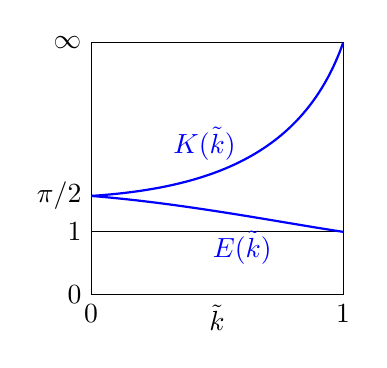
\begin{tikzpicture}[scale=0.8]
  \draw (0,0) rectangle (4,4);
  \draw (0,1.0) -- (4,1.0);
  \draw[thick,blue] (0,1.57) .. controls (2,1.7) and (3.4,2.3) .. (4,4);
  \draw[thick,blue] (0,1.57) .. controls (1.5,1.45) and (3,1.15) .. (4,1.0);
  \node[left] at (0,1.57) {$\pi/2$}; \node[left] at (0,1.0) {$1$}; \node[left] at (0,0) {$0$};
  \node[left] at (0,4) {$\infty$};
  \node[below] at (0,0) {$0$}; \node[below] at (4,0) {$1$}; \node[below] at (2,0) {$\tilde k$};
  \node[blue] at (1.8,2.4) {$K(\tilde k)$};
  \node[blue] at (2.4,0.75) {$E(\tilde k)$};
\end{tikzpicture}
\diagramcaption{The complete elliptic integrals $K(\tilde k)$ and $E(\tilde k)$.}
\end{diagram}

The nearest-neighbor correlation function is
\begin{equation}
  \ev{\sigma_{00}\sigma_{10}} = \ev{\sigma_{00}\sigma_{01}} =
  \begin{cases}
    \sqrt{1+\tilde k_>^{-1}}\left[\dfrac{1}{2} + (\tilde k_>-1)\dfrac{K(\tilde k_>)}{\pi}\right] & \text{for } T>T_c\\[10pt]
    \sqrt{1+\tilde k_<}\left[\dfrac{1}{2} - (\tilde k_<-1)\dfrac{K(\tilde k_<)}{\pi}\right] & \text{for } T<T_c .
  \end{cases}
\end{equation}
These are both $=1/\sqrt2$ at $T = T_c$.

C.N.~Yang: the spontaneous magnetization is
\begin{equation}
  M_{sp} = (1-\tilde k_<^2)^{1/8}\ \Rightarrow\ \beta = \frac{1}{8} .
\end{equation}
Via the relation $\bar\chi = \sum_{\mathbf r}\ev{\sigma_{\mathbf 0}\sigma_{\mathbf r}}_{\text{conn.}}$,
calculate the asymptotic behavior of $\bar\chi$ $\Rightarrow\gamma = \gamma' = 7/4$:
\begin{equation}
  \bar\chi\sim\begin{cases}\dfrac{1}{|T-T_c|^{\gamma}} & T>T_c\\[8pt] \dfrac{1}{|T-T_c|^{\gamma'}} & T<T_c,\end{cases}
\end{equation}
and the critical decay at $T_c$:
\begin{equation}
  \ev{\sigma_{\mathbf 0}\sigma_{\mathbf r}}\sim\frac{1}{r^{d-2+\eta}} = \frac{1}{r^\eta},\qquad\text{where }\eta = \frac{1}{4} ;
\end{equation}
also $\delta = 15$, with $M\sim H^{1/\delta}\sgn(H)$ at $T_c$.

\subsubsection*{Summary of critical exponents in the 2D Ising model and comparison with Landau--Ginzburg and MFT}

\begin{center}
\renewcommand{\arraystretch}{1.25}
\begin{tabular}{lcc}
  & LG/MFT & 2D Ising\\ \hline
  $\alpha,\alpha'$ & 0 (disc.) & 0 (log div.)\\
  $\beta$ & $1/2$ & $1/8$\\
  $\gamma,\gamma'$ & 1 & $7/4$\\
  $\nu,\nu'$ & $1/2$ & 1\\
  $\eta$ & 0 & $1/4$\\
  $\delta$ & 3 & 15
\end{tabular}
\end{center}
Later, we will show that these critical exponents depend on only two fundamental exponents, $y_T$, the
thermal exponent, and $y_h$, the magnetic exponent.
